
\begin{figure*}[!ht]
    \centering
    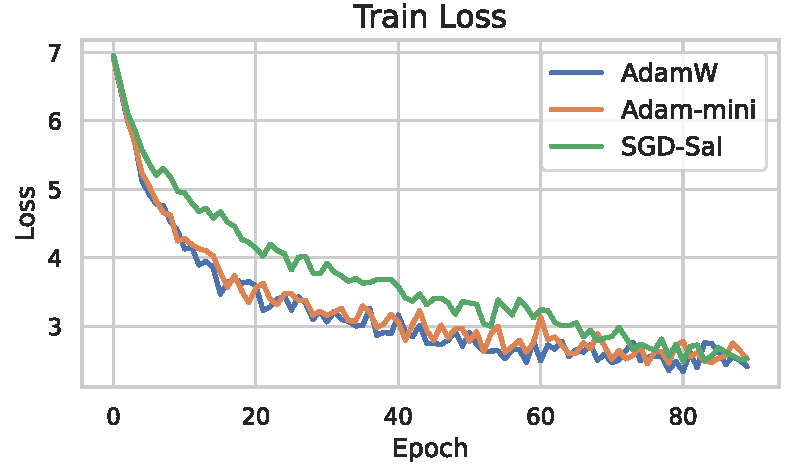
\includegraphics[width=0.33\linewidth]{images/vit_trainloss.pdf}
    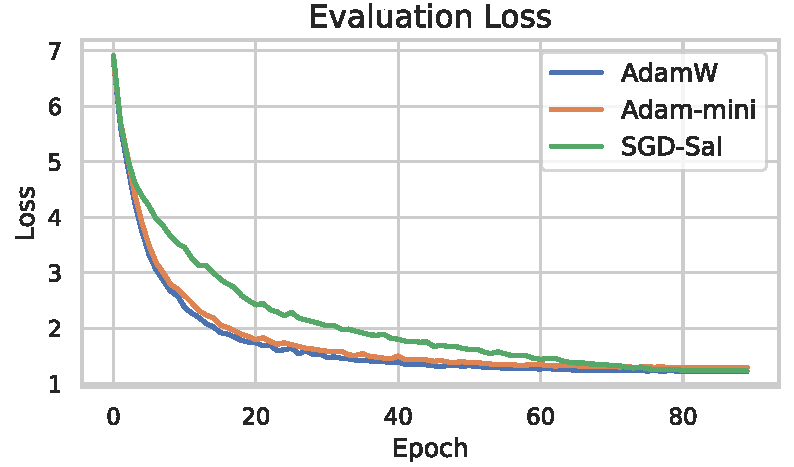
\includegraphics[width=0.33\linewidth]{images/vit_evalloss.pdf}
    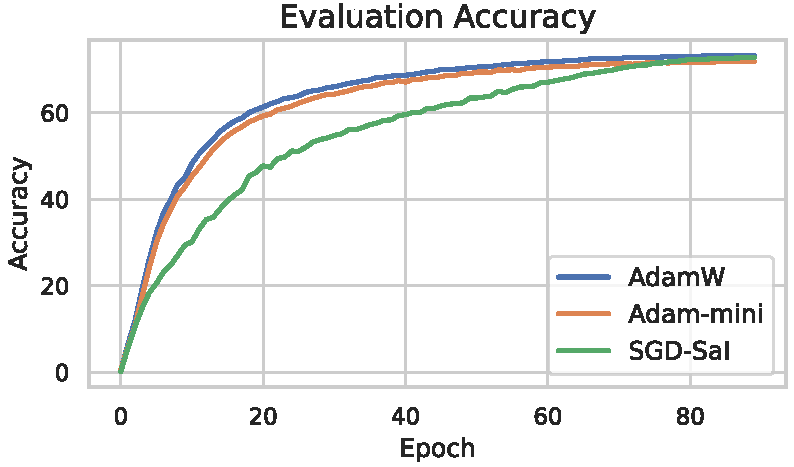
\includegraphics[width=0.33\linewidth]{images/vit_evalacc.pdf}
    \caption{This figure displays the training and evaluation loss and accuracy of the ViT on ImageNet1k). Although our method has a slower convergence speed, we can still achieve comparable performance by the end of the training process. Additionally, our approach is designed to have a lower memory footprint and a faster optimization speed. }
    \label{fig:vit_loss_acc_across_time}
\end{figure*}

\begin{figure}[!ht]
    \centering
    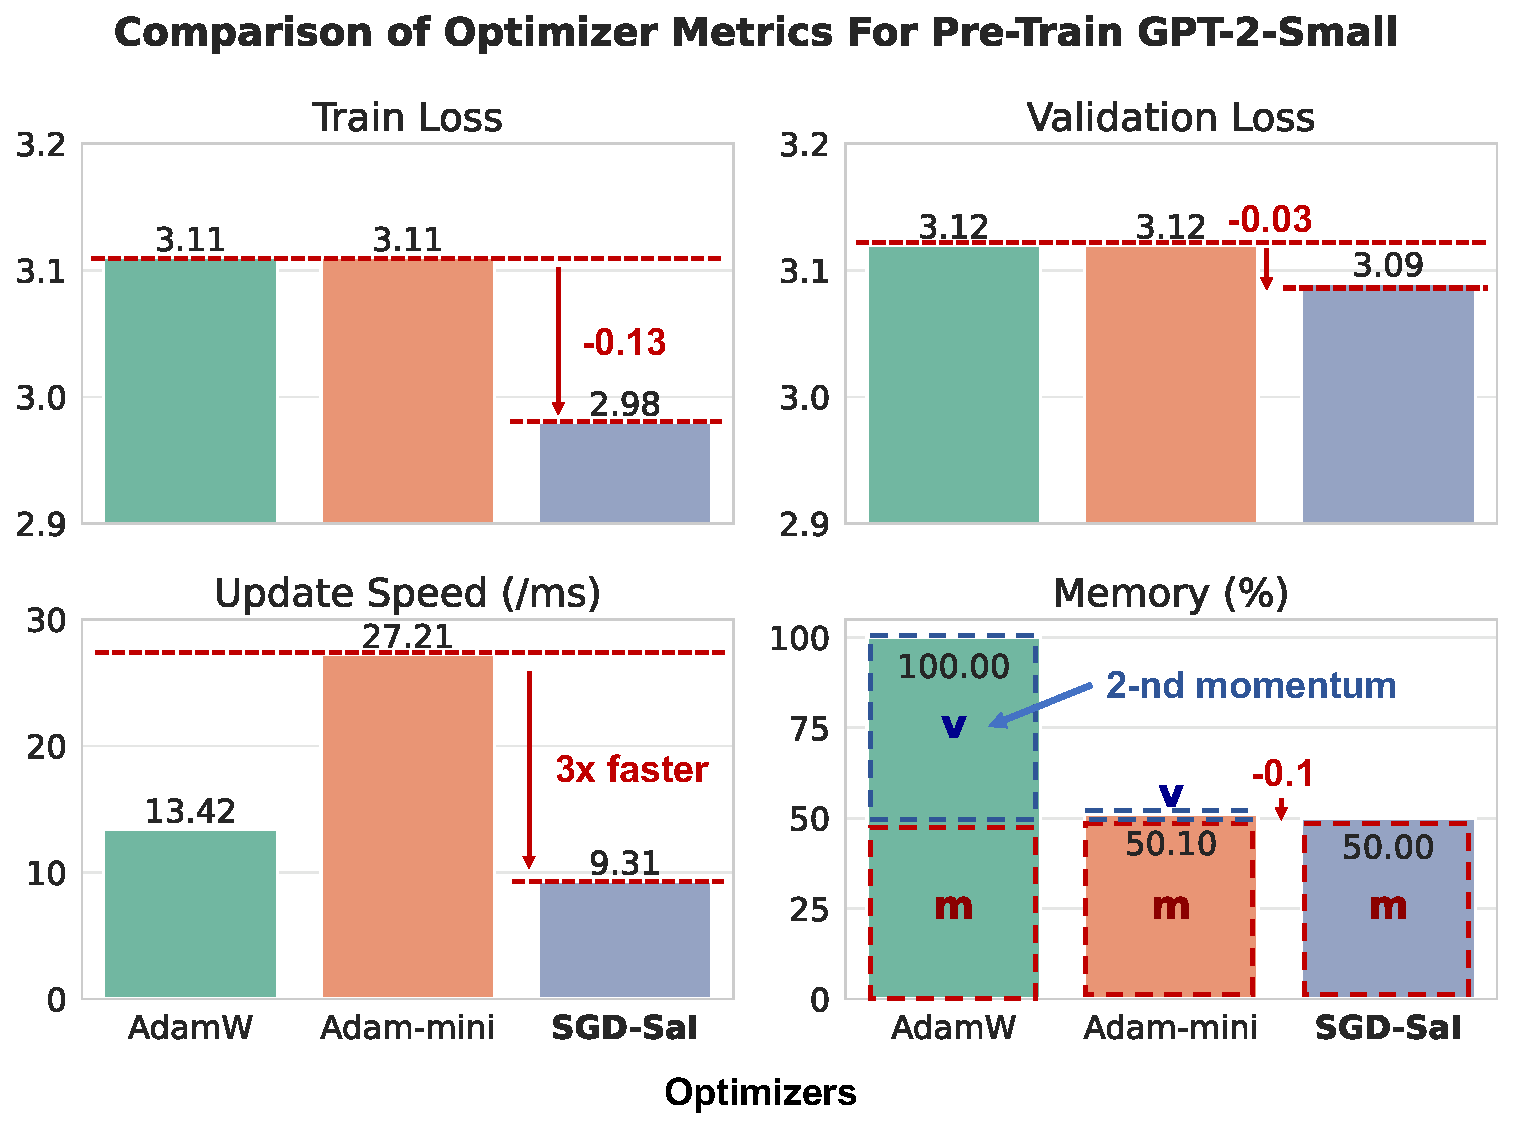
\includegraphics[width=\linewidth]{images/gpt2_exp_results.pdf}
    \caption{Metrics comparison of optimizers (AdamW, Adam-mini, and SGD-SaI) during pre-training of GPT-2 Small. The figure includes four subplots: (a) Train Loss shows that SGD-SaI achieves the lowest train loss, outperforming Adam-mini by 0.13. (b) Validation Loss illustrates a slight improvement in SGD-SaI with a reduction of 0.03 compared to Adam-mini. (c) Update Speed highlights that SGD-SaI is three times faster than Adam-mini, with AdamW showing moderate performance. (d) Memory Usage indicates that AdamW consumes 100\% memory, while both Adam-mini and SGD-SaI utilize approximately half, demonstrating better efficiency. Annotated values provide clarity on performance metrics, with red highlights emphasizing improvements from Adam-mini.}
    \label{fig:optimizer_metrics_comparison}
\end{figure}



\section{Experiments}
\label{sec:results}

This section evaluates our method through several tasks, including pre-training for Large Language Model (LLM) and Vision Transformer (ViT), Parameter-Efficient Fine-Tuning (PEFT) tasks on LLM and Diffusion Model (DM), and traditional Convolutional Neural Network (CNN) tasks. The specific tasks are outlined as follows:

\begin{itemize}
    \item \textbf{Large Language Model(Transformer Decode Only)} We pre-train GPT-2~\cite{radford2019language} on OpenWebText~\cite{Gokaslan2019OpenWeb}. We profile the optimizer state tensors' memory usage and optimizer step time for GPT-2-XL(1.5B) and LLM2-7B.
    \item \textbf{Vision Transformer} We investigate the Vision Transformer (ViT/S-16)~\cite{dosovitskiy2021imageworth16x16words} on the ImageNet-1k dataset~\cite{deng2009imagenet} for image classification tasks.  We profile the optimizer state tensors' memory usage and optimizer step time for ViT-H/14.
    \item \textbf{Parameter-Efficient Fine-Tuning (PEFT) LoRA} Furthermore, we explore Parameter-Efficient Fine-Tuning (PEFT) tasks for GPT-2 LoRA\cite{hu2021lora} fine-tuning on the E2E~\cite{novikova2017e2e} dataset and Diffusion Model fine-tuning to capture visual concepts. For image classification, we report the top-1 validation accuracy, while for Large Language Model (LLM) fine-tuning tasks, to evaluate the results of the fine-tuning, we report metrics such as BLEU~\cite{papineni2002bleu}, NIST~\cite{doddington2002automatic}, MET~\cite{banerjee2005meteor}, ROUGE-L~\cite{lin2004rouge}, and CIDEr~\cite{vedantam2015cider}. For all these metrics, higher scores indicate better performance. Additionally, we perform qualitative evaluations for the Diffusion Model (DM) fine-tuning task.
    \item \textbf{Convolutional Neural Networks (CNNs).} We study ResNet-18 (11M parameters) on the CIFAR-10 dataset, and architectures from NATS-Bench~\cite{dong2021nats} on CIFAR-10, CIFAR-100, and ImageNet16-120~\cite{krizhevsky2009learning, chrabaszcz2017downsampled}. All these are image classification tasks, and we report the top-1 test accuracy as the evaluation metric. 
\end{itemize}


\subsection{LLM Pre-train}\label{sec:exp:pretrain_llm}
\textbf{Setups.} 
We pre-train GPT-2-Small (125M)~\cite{radford2019language} on OpenWebText~\cite{Gokaslan2019OpenWeb}. We compare SGD-SaI with AdamW~\cite{loshchilov2019decoupled} and Adam-mini~\cite{zhang2024adamminiusefewerlearning}. We follow the same settings as described in the previous study~\cite{zhang2024adamminiusefewerlearning}. We analyse the loss metrics for each optimizer. 

For large-scale LLMs, we provide profiling results focusing on memory usage and wall-clock time during the optimizer step for GPT-2-XL (1.5B parameters) and Llama-2 (7B parameters). Due to resource constraints, these results are limited to the optimizer step time and do not encompass full training runs.
We compare SGD-SaI with SGDM, AdamW, Adam~\cite{kingma2014adam}, Adam-mini, and Prodigy~\cite{mishchenko2023prodigy}.
The reported metrics include memory usage of the state tensors and the time costs associated with the optimizer steps. All results were obtained using a single NVIDIA A100 (80GB).


\textbf{Results.} 
Figure~\ref{fig:optimizer_metrics_comparison} compares optimizers (AdamW, Adam-mini, and SGD-SaI) during pre-training of GPT-2-Small across multiple metrics. While SGD-SaI demonstrates a slightly slower initial convergence speed compared to the Adam family optimizers due to its design, it achieves superior final convergence with a lower training loss (outperforming Adam-mini by 0.13). Similarly, validation loss shows a marginal improvement, with SGD-SaI reducing it by 0.03 compared to Adam-mini.

\textbf{Efficiency.}
\textit{For the GPT-2-Small pre-training task.} Regarding update speed, SGD-SaI demonstrates a significant advantage, being three times faster than Adam-mini in parameter updates and outperforming AdamW. Furthermore, the memory efficiency of SGD-SaI is noteworthy—it consumes only half the memory required by AdamW while maintaining performance comparable to Adam-mini, which employs intricate partitioning strategies. Unlike Adam-mini, which requires complex parameter partitioning (eg. users need to manually transform the Pytorch default partitions like the combined QKV block into separate Q, K and V blocks.), SGD-SaI achieves similar or better results using the default PyTorch partitioning, highlighting its simplicity and efficiency.
\textit{For the untrained models.} By design, the state tensors for Adam and AdamW are approximately twice the size of the gradient, while Prodigy’s state tensors are roughly four times larger. In contrast, SGD-SaI has state tensors of the same size as standard SGDM. This effectively reduces memory usage by up to 75\% compared to Prodigy and by 50\% compared to Adam(W). The detailed discussion can be found in the Appendix~\ref{sec:sup:optimizer_breakdown}. As shown in Table~\ref{table:llm_profiled_performance}, SGD-SaI maintains a manageable memory footprint, enabling it to work with large models like Llama-2 (7B) without running into out-of-memory (OOM) errors. In contrast, other optimizers, such as AdamW and Prodigy, exceed available memory limits at this model size, highlighting the scalability challenges posed by memory-intensive optimizers when dealing with long context lengths in LLMs.
Adam-Mini requires a partitioning strategy for different parameter groups while adjusting the learning rate adaptively at each time step. This increases memory usage and computational cost as different groups can not update simultaneously. For models larger than 1 billion parameters, the performance gains from Adam-Mini decrease by approximately 45\%, while the reduction achieved with SGD-SaI remains around 50\%.


\begin{table}[!ht]
\centering
\small % Reduce font size for CVPR two-column format
\setlength{\tabcolsep}{6pt} % Reduce column padding
\renewcommand{\arraystretch}{1.3} % Adjust row height
\resizebox{0.9\columnwidth}{!}{
\begin{tabular}{l|l|l|l}
\hline
Model & Method & State Mem (GB) & Wall Time (ms) \\ \hline
\multirow{6}{*}{GPT2-1.5B} 
    & SGDM        & 5.93  & 41.0 $\pm$ 12.0 \\
    & AdamW       & 11.86  & 138.0 $\pm$ 6.0 \\
    & Adam        & 11.86  & 145.0 $\pm$ 7.0 \\
    & Prodigy     & 23.72  & 360.0 $\pm$ 45.0 \\
    & Adam-Mini   & 6.52  & 223.0 $\pm$ 2.0 \\
    & \textbf{SGD-SaI(ours)}    & 5.93                        & 68.0 $\pm$ 21.0 \\ \hline
\multirow{6}{*}{Llama2-7B} 
    & SGDM        & 25.15                       & 100.0 $\pm$ 20.0 \\
    & AdamW       & 49.48                       & OOM \\
    & Adam        & 49.48                       & OOM \\
    & Prodigy     & 98.96                       & OOM \\
    & Adam-Mini   & 27.21                       & 421.0 $\pm$ 22.0 \\
    & \textbf{SGD-SaI(ours)}     & 25.15                       & 180.0 $\pm$ 30.0 \\ \hline
\end{tabular}
}
\caption{The efficiency metrics of various models with different optimizers were evaluated using an A100-80GB GPU. The table above summarizes the results, which include the tensor memory usage and wall-clock time (optimization step time measured in milliseconds) for each model-optimizer configuration. For the large language models (LLMs), experiments were conducted with a context length of 1024 and a batch size of 1. All models were profiled in full (FP32) precision.}
\label{table:llm_profiled_performance}
\end{table}

\subsection{ViT Pre-train}\label{sec:exp:pretrain_vit}
\textbf{Setups.} We pre-train ViT-S/16~\cite{dosovitskiy2021imageworth16x16words} on the ImageNet1k dataset~\cite{deng2009imagenet} for the image classification task.
We compare SGD-SaI with AdamW~\cite{loshchilov2019decoupled} as well as popular optimizers including SGDM, Adam~\cite{kingma2014adam}, Adam-mini~\cite{zhang2024adamminiusefewerlearning} and Prodigy~\cite{mishchenko2023prodigy}.
After conducting a grid search within the same hyperparameter range, we compare the optimiser results. We report the peak and mean of the top-1 validation accuracy to evaluate their generalisation ability and sensitivity to hyperparameter changes. Detailed hyperparameters are in Appendix~\ref{sec:sup:vit_gs_details}.

Due to the intensive computational power requirements for the ViT variants during the grid search, we cannot provide the complete training results. Instead, we follow the same procedure outlined in Section~\ref{sec:exp:pretrain_llm} and present only the profiling results regarding memory usage and wall-clock time during the optimizer step for ViT-S/16 and ViT-H/14. Additionally, we compare SGD-SaI with SGDM, AdamW, Adam, Adam-mini, and Prodigy.
All results were obtained using a single NVIDIA A100 with 80GB of memory.


\textbf{Results.} 
We report peak performance under the best hyperparameters, averaging results over three random seeds, and present the mean and standard deviation (see Table~\ref{table:vit_results}). Our simple re-scaling strategy significantly boosts SGDM's performance from 63.80 to 72.92, nearly matching AdamW's 73.04. Meanwhile, the recent SOTA optimizer Prodigy achieves a slightly higher peak at 73.24, though it requires additional one-time memory usage. We will discuss these results further in later sections. Notably, our approach achieves the lowest standard deviation (0.07) across three random seeds, compared to Prodigy’s second-lowest at 0.21, highlighting the stability of our method during training.

In addition, we examine average performance across the hyperparameter search grid using a rest setting that deviates from the best hyperparameters as a tweaked version. Under these conditions, we observe that most previous methods, including AdamW, struggle significantly, leading to dramatic drops in average performance. For example, AdamW, despite being an update over SGD intended to improve robustness to hyperparameters, achieves only 37.21 with a standard deviation of 35.43. In contrast, our method maintains overall performance, achieving an average of 57.55 with a much lower variance (standard deviation of 18.46). Prodigy, a parameter-free optimizer not designed to adjust learning rate and weight decay, fails to converge when these hyperparameters are modified; thus, we exclude it from this part of the comparison for fairness.

\begin{table}[!ht]
\resizebox{0.96\columnwidth}{!}{
\begin{tabular}{lcc}
\hline
\textbf{Optimizer} & \textbf{Peak@top1 (\%)}      & \textbf{Avg@top1 (\%)}        \\ \hline
SGDM               & 63.80 $\pm$ 0.35             & 14.33 $\pm$ 19.38             \\
Adam               & 61.56 $\pm$ 0.93             & 20.93 $\pm$ 22.05             \\
Adam-Mini           & 72.29 $\pm$ 0.43             & 36.65 $\pm$ 35.39             \\
AdamW              & \underline{73.04} $\pm$ 0.31 & \underline{37.21} $\pm$ 35.43 \\ \hline
Prodigy            & \textbf{73.24} $\pm$ 0.21    & N/A                           \\ \hline
SGD-SaI(Ours)    & 72.92 $\pm$ \textbf{0.07}             & \textbf{57.55} $\pm$ \textbf{18.46}    \\ \hline
\end{tabular}
}
\caption{Comparison of peak and average top-1 validation accuracy on ImageNet-1k for ViT-S/16 trained from scratch. Each optimizer's performance is evaluated over a hyperparameter search space, reporting the highest accuracy (Peak@top1) and the average accuracy (Avg@top1) across all trials. Results are averaged over three seeds, with standard deviations for statistical analysis. Our method achieves significantly higher robustness to hyperparameter variations, maintaining a high average performance (57.55\%) and outperforming other optimizers by at least 20\%.}
\label{table:vit_results}
\end{table}


Our method demonstrates superior robustness and effectiveness in training ViT-S/16 models from scratch on ImageNet-1k, outperforming previous optimizers across peak and average performance metrics. While alternative optimizers like AdamW and Prodigy achieve high peak accuracy, their performance drops significantly under hyperparameter variations, highlighting their sensitivity. In contrast, our approach maintains a stable and high average accuracy across diverse hyperparameter settings with minimal standard deviation. It underscores its resilience to hyperparameter tuning and potential for more efficient and reliable model training in real-world applications. This stability makes our method particularly suitable for scenarios where hyperparameter tuning is constrained, offering a consistent and robust solution for training large models.

Although our method does not utilize adaptive gradient adjustments, it achieves a stable and steady learning pace, ultimately reaching a comparable performance, as shown in Figure~\ref{fig:vit_loss_acc_across_time}. Empirically, this stability arises from our preconditioned learning rate, which ensures each step is well-controlled and converges reliably with sufficient training steps. In contrast, Adam-family optimization methods often achieve faster convergence but are prone to being trapped in suboptimal minima due to their aggressive adaptivity.

\textbf{Efficiency.} 
As shown in Table~\ref{table:vit_profiled_performance}, our method achieves a wall-clock time for optimizer steps comparable to SGDM, while being significantly faster than Adam-mini, Adam(W), and Prodigy. We must note that we present the wall clock time for each optimizer step rather than the total runtime. We did not rely on the grid search results to report the total runtime because all grid search experiments were conducted on a cluster. Due to complex factors, such as the cluster's I/O bottleneck and network congestion, distributed training can be considerably slowed down. We chose to maintain the same settings and device while profiling the LLM. Regarding memory usage, similar trends were observed during the pre-training of GPT-2 Small. For example, the ViT-H/14-0.66B model uses only 2.42 GB of memory with SGD-SaI, compared to 4.86 GB with AdamW and 9.70 GB with Prodigy. Our method reduces memory consumption by 50\% compared to Adam(W) and by 75\% compared to Prodigy. Further empirical analysis can be found in App.~\ref{sec:sup:optimizer_breakdown}.

\begin{table}[!ht]
\centering
\small % Reduce font size for CVPR two-column format
\setlength{\tabcolsep}{6pt} % Reduce column padding
\renewcommand{\arraystretch}{1.3} % Adjust row height
\resizebox{0.9\columnwidth}{!}{
\begin{tabular}{l|l|l|l}
\hline
Model & Method & State Mem (GB) & Wall Time (ms) \\ \hline
\multirow{6}{*}{ViT-S/16(0.0229B)} 
    & SGDM        & 0.08  & 7.9 $\pm$ 0.3 \\
    & AdamW       & 0.17  & 45.0 $\pm$ 8.0 \\
    & Adam        & 0.17 & 50.0 $\pm$ 1.5 \\
    & Prodigy     & 0.33  & 78.0 $\pm$ 0.0 \\
    & Adam-Mini   & 0.08  & 84.0 $\pm$ 5.0 \\
    & \textbf{SGD-SaI(ours)}   & 0.08 & 12.4 $\pm$ 0.2 \\ \hline
\multirow{6}{*}{ViT-H/14(0.66B)} 
    & SGDM        & 2.42  & 40.0 $\pm$ 1.0 \\
    & AdamW       & 4.86  & 124.0 $\pm$ 4.0 \\
    & Adam        & 4.86  & 127.0 $\pm$ 2.0 \\
    & Prodigy     & 9.70  & 260.0 $\pm$ 3.0 \\
    & Adam-Mini   & 2.54  & 220.0 $\pm$ 20.0 \\
    & \textbf{SGD-SaI(ours)}    & 2.42                        & 54.0 $\pm$ 13.0 \\ \hline
\end{tabular}
}
\caption
{We maintain the same settings as in Table~\ref{table:llm_profiled_performance}. We ensure a comparable memory footprint to SGDM, while keeping the optimizer step time controlled, resulting in a performance that is \textbf{4-6 x faster than} Adam-mini.}
\label{table:vit_profiled_performance}
\end{table}

\begin{figure*}[!ht]
    \centering
    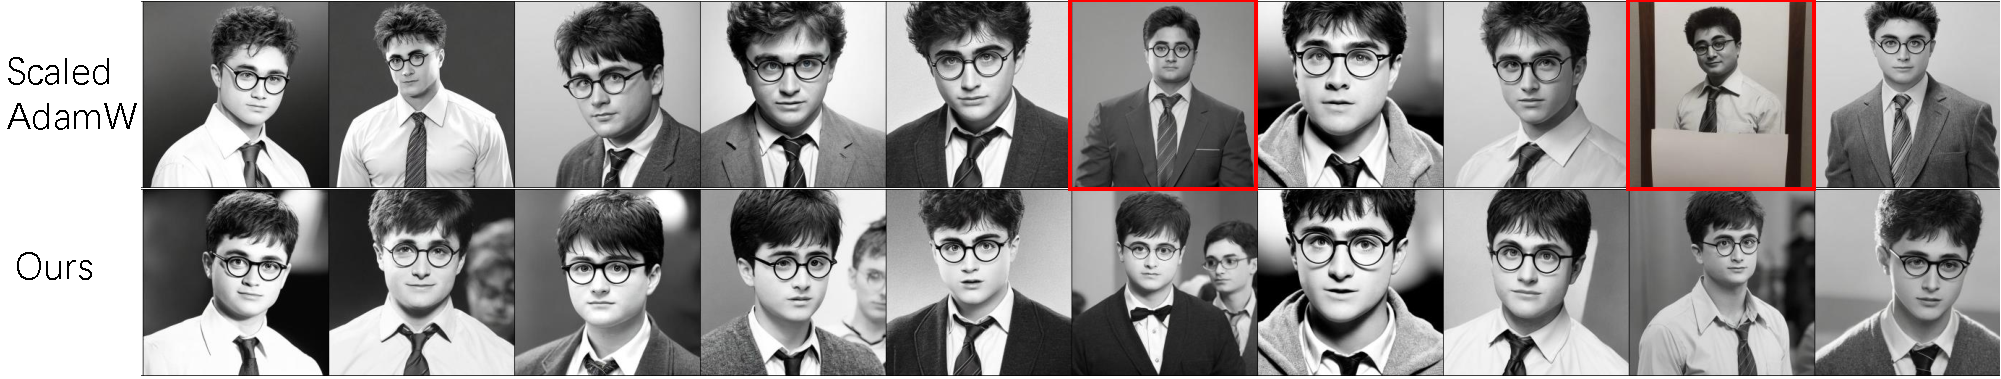
\includegraphics[width=0.9\textwidth]{images/mixofshow.pdf}     
    %\vspace{-3mm}
    \caption{Generation results for prompt “a pencil sketch of ⟨Vpotter⟩” by Mix-of-Show model with \textbf{scaledAdamW optimizers(up)} and \textbf{our optimizer(down)}. Our method generates photos that better capture the prompt and align with visual concepts from training samples; At the same time, previous SOTA-scaled AdamW has some significant bad cases that do not follow the prompt, we marked them with a red bounding box.}
    \label{fig:mix_of_show}
    \vspace{-3mm}
\end{figure*}

\begin{figure*}[!ht]
    \centering
     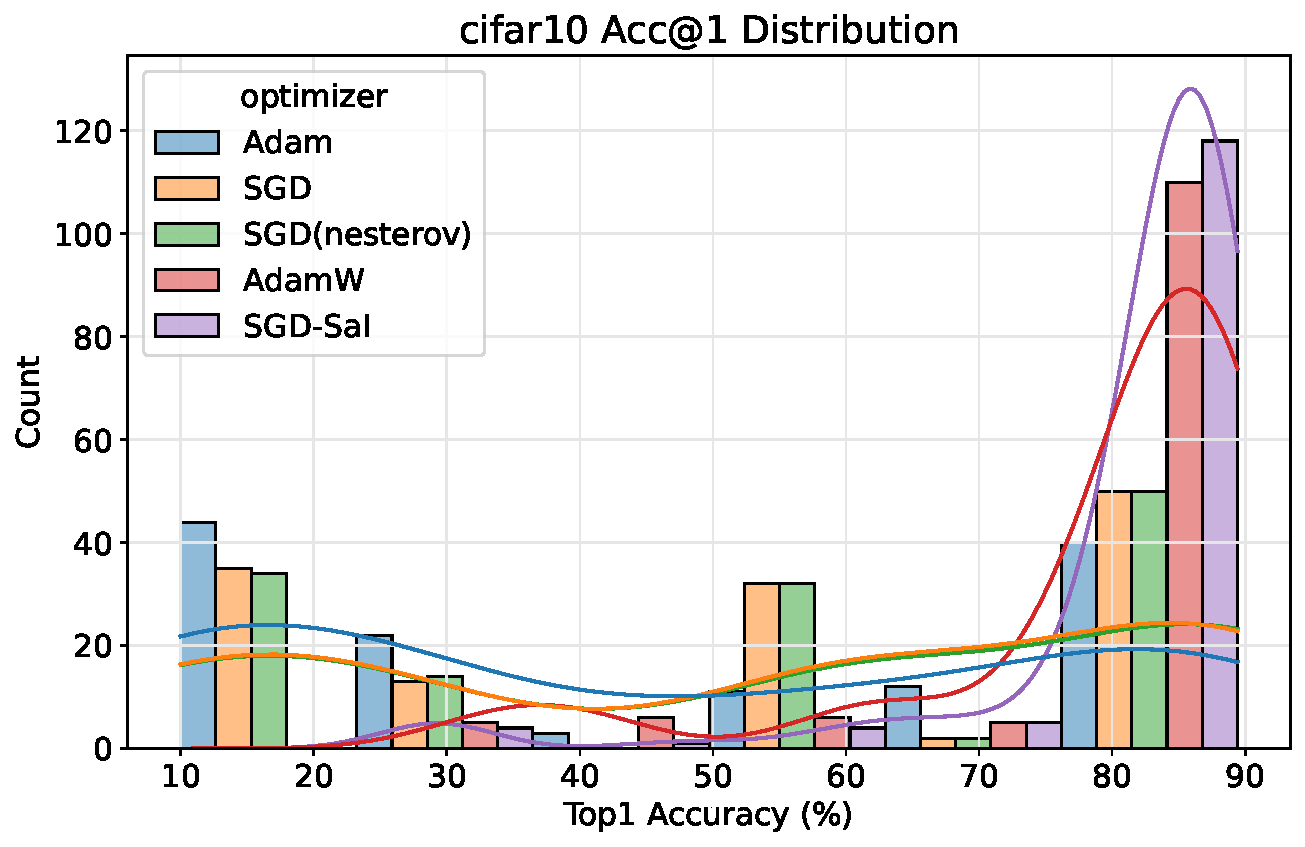
\includegraphics[width=.32\textwidth]{images/SSS_cifar10_valid_acc1_max_distribution.pdf}
     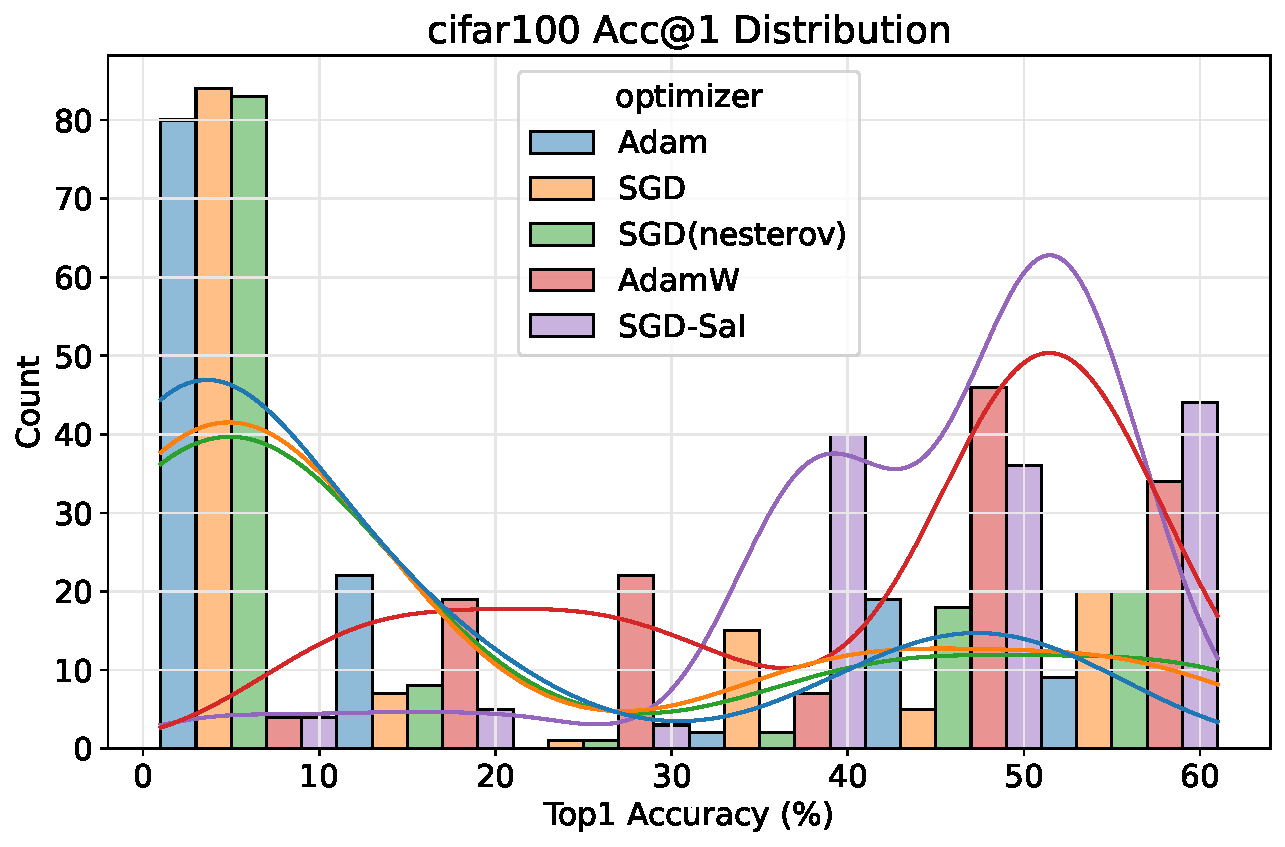
\includegraphics[width=.32\textwidth]{images/SSS_cifar100_valid_acc1_max_distribution.pdf}
     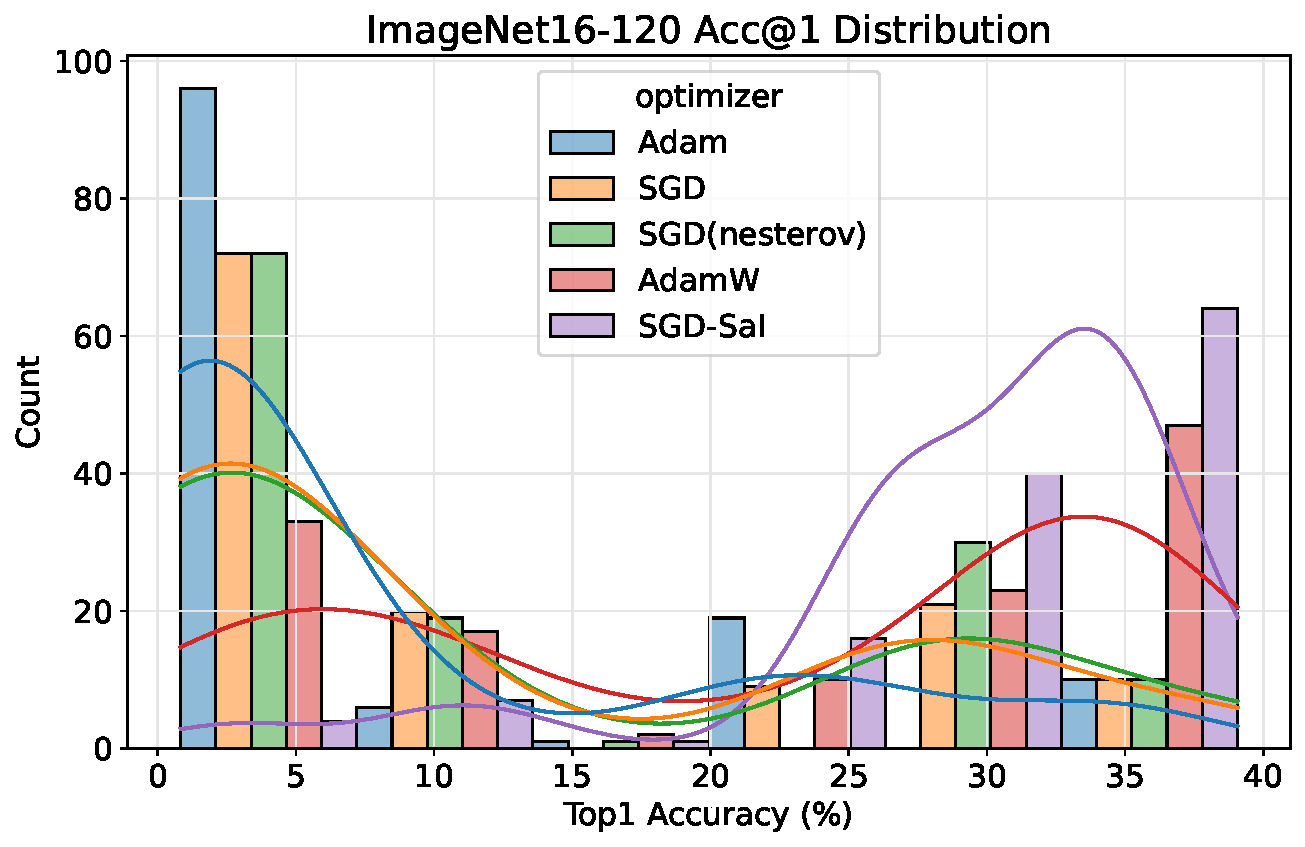
\includegraphics[width=.32\textwidth]{images/SSS_ImageNet16-120_valid_acc1_max_distribution.pdf}
    \caption{These figures show the accuracy distributions of eleven architectures trained on different optimizers using the same hyperparameter candidates.  This row presents the top-1 evaluation accuracy distributions on CIFAR-10, CIFAR-100 and ImageNet16-120. The curves in those histograms are the results of kernel density estimation (KDE).}
    \label{fig:fig_sss_performance_distribution_histogram}
\end{figure*}


\subsection{Parameter Efficient Fine Tuning: PEFT}\label{sec:exp:finetune_peft}
We primarily consider PEFT tasks on LLM fine-tuning and the Diffusion Model fine-tuning. 

\subsubsection{LLMs Parameter Efficient Fine-tuning}

\textbf{Setup.} 
We fine-tune the GPT-2 model using the E2E dataset ~\cite{novikova2017e2e}. The current state-of-the-art (SOTA) methods include scaled-SGD and scaled-AdamW from ~\cite{zhang2024riemannian}, which adjust the learning rates for parameters $A$ and $B$ with a Riemannian preconditioner. Our primary comparison is between SGD-SaI and these methods, along with Adam-mini. To evaluate the results of the fine-tuning, we report metrics such as BLEU~\cite{papineni2002bleu}, NIST~\cite{doddington2002automatic}, MET~\cite{banerjee2005meteor}, ROUGE-L~\cite{lin2004rouge}, and CIDEr~\cite{vedantam2015cider}. For all these metrics, higher scores indicate better performance.

\textbf{Results.} 
We adopted the same experiment setting to investigate whether our methods suit LoRA Training~\cite{hu2021lora}. We set the default learning rate to \(1e-3\) and weight decay to \(1e-2\). Empirically, we observe that SGD-SaI outperforms previous state-of-the-art (SOTA) scaled optimizers and unscaled ones. Table~\ref{tab:lora_scores} presents surprising results regarding the final scores for LoRA fine-tuning of the GPT-2 medium model with a rank of 4 on the E2E natural language generation tasks. With this simple precondition on SGDM, our method performs significantly better than the previous SOTA strategy using rescaled SGD. Furthermore, our approach exhibits a substantial improvement over AdamW in fine-tuning the GPT-2 architecture, even without meticulous tuning and searching for hyperparameters.

\begin{table}[!ht]
\centering
\resizebox{\columnwidth}{!}{
\begin{tabular}{l|c|c|c|c|c}
\hline
\textbf{Method} & \textbf{BLEU} & \textbf{NIST} & \textbf{MET} & \textbf{ROUGE-L} & \textbf{CIDEr} \\ \hline
SGD\textsubscript{\(r=4\)} & 66.6 & 8.54 & 44.2 & 68.2 & 2.32 \\ 
scaled SGD\textsubscript{\(r=4\)} & 69.2 & 8.71 & 46.3 & 70.9 & 2.48 \\ 
AdamW\textsubscript{\(r=4\)} & 68.9 & 8.69 & 46.5 & 71.3 & 2.51 \\
Adam-Mini\textsubscript{\(r=4\)} & 68.7 & 8.66 & 46.3 & 71.1 & 2.50 \\
scaled AdamW \textsubscript{\(r=4\)} & 69.6 & 8.77 & 46.6 & 71.8 & 2.52   \\ \hline
SGD-SaI (ours)\textsubscript{\(r=4\)} & \textbf{69.9} & \textbf{8.81} & \textbf{46.7} & \textbf{72.1} & \textbf{2.53} \\
\end{tabular}
}
\caption{This table presents scores for LoRA fine-tuning of GPT-2 medium model on E2E Natural Language Generation (NLG) challenge with different optimizers. SGD-SaI outperforms all scaled and unscaled optimizers on all evaluation metrics. In particular, our method closes the performance gap between SGD and AdamW and reveals its effectiveness in performing block-wise scaling.}

\label{tab:lora_scores}
\end{table}


\subsubsection{DMs Parameter Efficient Fine-tuning}

\textbf{Setup.} 
Using the diffusion model, we extend our experiments to include LoRA fine-tuning on image generation tasks. Specifically, we utilize the ChilloutMix model to address real-world concepts, following the same approach outlined in Mix-of-show \cite{gu2024mix, zhang2024riemannian}. Additionally, we compare our method with the state-of-the-art (SOTA) optimized approach using scaled-AdamW~\cite{zhang2024riemannian}. To evaluate the images generated by the diffusion model, we conduct a qualitative assessment to determine which method captures visual concepts more effectively.

\textbf{Results.}
Face generation is a challenging task; the model should understand the visual concept of a specific person's face based on its prompt text. Here, we set the learning rate as default 0.1, a large enough default value. We observed as Fig.~\ref{fig:mix_of_show}, even without carefully tuning the learning rate, our scaled methods have shown a significantly better ability to capture the visual concept of \textbf{potter} than the previous SOTA scaled approach scaled-AdamW~\cite{zhang2024riemannian}. It should be verified that our optimizer has better parameters robustness on training and leads to better convergence in final performance; this should be an essential benefit for the practical use of the optimizer. 




\subsection{Convolutional Neural Network(CNN)} \label{sec:exp:pretrain_cnn} 

\textbf{Setup.} 
We follow a similar approach to Section~\ref{sec:exp:pretrain_vit} for evaluating CNN models. A grid search is performed on ResNet18~\cite{he2015deepresiduallearningimage} using the CIFAR-10 dataset, and across various architectures from NATS-Bench~\cite{dong2021nats} on CIFAR-10, CIFAR-100, and ImageNet16-120~\cite{krizhevsky2009learning, chrabaszcz2017downsampled}. All tasks involve image classification. We compare SGD-SaI with traditional optimizers (SGD and Adam-family) and report top-1 test accuracy. Details of the grid search experiments are provided in Appendix~\ref{see:sup:cnn_gs_details}.

\textbf{Results.} 
Figure~\ref{fig:fig_vit_cnn_performance_3d_surface} (left graph) presents the performance of ResNet18. Our method achieves a peak accuracy of 95.36\%, which not only surpasses that of Adam(W) and SGD but also shows greater stability. 
In addition, we evaluated a range of search spaces, including datasets such as CIFAR-10, CIFAR-100, and ImageNet16-120, as well as architectures of varying sizes. We conducted a grid search across eleven architectures, testing three learning rates and four weight decay values. The distribution of top-1 accuracies is illustrated in Fig.~\ref{fig:fig_sss_performance_distribution_histogram}, which demonstrates the stability of our method across different architectures and hyperparameter settings. 
Our approach results in models with lower standard deviations and higher mean accuracies, indicating enhanced stability and generalization. These findings highlight the robustness of our method across various CNN architectures.





